\documentclass[../Master.tex]{subfiles}
\begin{document}
\begin{multicols*}{2}
	\section{Reaction rate}
	Is always true that:
	\[
		r = \frac{dx}{dt} = \frac{1}{\nu _{B} } \frac{dCb}{dt}
	\]

	\section{Advance coefficient}

	\subsection{Adimensional advance coefficient}
	\begin{gather*}
		g = \frac{C_{A}^0 - C_{A}}{C_{A}^0} \\
		g = \frac{x}{C_{A}^0} \quad 0 \leq g \leq 1 \\
		C_{A} = C_{A}^0(1 - g)
	\end{gather*}
	\section{First order reactions}
	\subsection{Rate expression}
	\begin{center}
		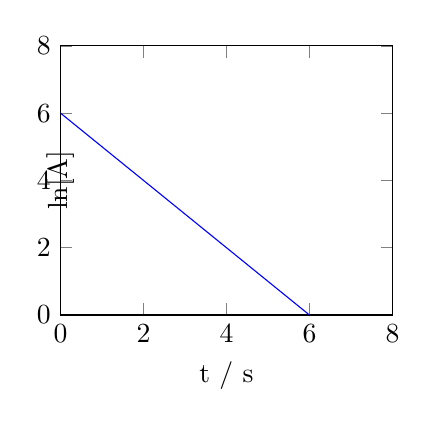
\begin{tikzpicture}
			\begin{axis}[
					height=5cm,
					xmin=0, xmax=8, % x scale
					ymin=0, ymax=8, % y scale
					domain=0:10,
					samples=101,
					smooth,
					no markers,
					% x label style={at={(axis description cs:0.5,-0.1)},anchor=north},
					y label style={at={(axis description cs:0.07,0.5)}}, xlabel={t / s},
					ylabel={ln[A]}] ] \addplot {-x + 6};
			\end{axis}
		\end{tikzpicture}
		\vspace{-1cm}
	\end{center}
	\begin{gather*}
		A \to P \\
		r = -\frac{dC_{A}}{dt} = k[A]\\
		- \ln C_{A} + \ln C_{0A} = kt\\
		\ln (\frac{C_{A}^0 }{C_{A}}) = e^{-kt}\\
		\frac{C_{A} }{C_{A}^{0} } = e^{-kt}	\end{gather*}

	\subsubsection{Alternative rate expression}
	One can use g to express the rate:
	\begin{gather*}
		Check TickTick
	\end{gather*}

	\subsection{Half-life time}
	\[
		t_{\frac{1}{2}} = \frac{\ln2}{k} \quad [s^{-}]
	\]
	In theory one can calculate the reactant concentration
	\begin{gather*}
		\ln \left( \frac{C_{A}^0 }{C_{A} } \right) = knt_{1 / 2}\\
		kt_{1 / 2} = \ln 2 \implies C_{A} = \frac{C_{A}^0 }{2^n}
	\end{gather*}

	\subsection{Life time}
	It is define as the time needed to reduce the reactant concentrationby a factor of \( \frac{1}{e} \)

	\begin{gather*}
		C_{A}= \frac{C_A^0}{e}\\
		\frac{C_{A}}{C_{A}^0} = e^{-1}\\
		kt = 1 \implies \tau = t = \frac{1}{k} \\
		C_{A} = C_{A}^{0} e^{- t / \tau }
	\end{gather*}

	\section{Second order reactions}
	\subsection{Unimolecolar reaction}
	\begin{gather*}
		r = \frac{dC_{A}}{dt} = k[A]^{2} \\
		\frac{1}{C_{A} } - \frac{1}{C_{A} ^{0}} = kt
	\end{gather*}
	\subsubsection{Half-life time}
	\[
		t_{\frac{1}{2}} = \frac{1}{C_{A} ^{0}k}
	\]

	\subsection{Bimolecolar reaction}
	\begin{gather*}
		r = - \frac{dC_{A}}{dt} = - \frac{dC_{B}}{dt} = \frac{dx}{dt} = k[A][B] \\
		\frac{1}{C_{A} ^{0} - C_{B} ^{0} }~\ln\left[\frac{(C_{A} ^{0} - x)C_{B} ^{0} }{(C_{B} ^{0} - x) C_{A} ^{0} }\right] = kt\\
		\frac{C_{B}}{C_{A}} = \frac{C_{B} ^{0} }{C_{A} ^{0} }e^{(C_{A} ^{0}-C_{B} ^{0}  )kt}
	\end{gather*}

	\subsubsection{Half-life time}
	\[
		t_{\frac{1}{2}} = \frac{1}{C_{A} ^{0} - C_{B} ^{0} k}~ ~  \ln\left(  \frac{2C_{A} ^{0} - C_{B}^{0} }{C_{A}^{0}} \right)
	\]

	\section{Zero order reactions}
	\begin{gather*}
		r = k\\
		C = C^0 - kt
	\end{gather*}
	\subsection{Half-life time}
	\[
		t_{\frac{1}{2}}  = \frac{1}{2}t_{f}
	\]
	\section{nth order reactions}
	\begin{gather*}
		r = k[A]^{n} \\
		\frac{1}{C^{n-1} } - \frac{1}{C^{0(n-1 )} } = (n-1)kt\\
	\end{gather*}
	\subsection{Half-life time}
	\[
		t_{\frac{1}{2}} = \frac{2^{n-1} -1 }{(C^{0} )^{n-1} k(n-1)}
	\]

	\section{Parallel reactions}
	In this condition A react with different velocity constant towards different
	products W,V and U.
	\begin{gather*}
		\ce{ A ->[{k_{1}}] U} \\
		\ce{ A ->[{k_{2}}] W} \\
		\ce{ A ->[{k_{3}}] V} \\
		r =  - \frac{dC_{A} }{dt} = k_{1}C_{A} + k_{2}C_{A} + k_{3}C_{A} = kC_{A}
	\end{gather*}

	Equation for the products can be written as:
	\begin{gather*}
		C_{U} - C_{U}^{0} = \frac{k_{1}C_{A}^{0}}{k}(1-e^{-kt})\\
		C_{V} - C_{V}^{0} = \frac{k_{2}C_{A}^{0}}{k}(1-e^{-kt})\\
		C_{W} - C_{W}^{0} = \frac{k_{3}C_{A}^{0}}{k}(1-e^{-kt})
	\end{gather*}
	k can be determined sperimentally from the relation between \( C_{A}  \) and time, in this case it would be a first order relation.
	Concentration of the products can be determined with sperimental methods. At this point the following system can be used:

	\begin{equation*}
		\begin{cases}
			k_{1} + k_{2} + k_{3} = k                  \\
			\frac{C_{U}}{C_{W} } = \frac{k_{1}}{k_{2}} \\
			\frac{C_{U} }{C_{V}} = \frac{k_{2}}{k_{3}}
		\end{cases}
	\end{equation*}

	\section{Consecutive reactions}
	\begin{gather*}
		\ce{ A ->[{k_{1}}] B ->[{k_{2}}]C}\\
	\end{gather*}
	This is the simpliest case, with all first order reactions
	\begin{gather*}
		r = -\frac{dC_{A}}{dt} = k_{1}C_{A}\\
		r = \frac{dC_{B}}{dt} = k_{1}C_{A} - k_{2}C_{B}\\
		r = \frac{dC_{C}}{dt} = k_{2}C_{B}
	\end{gather*}
	The $C_{C}$ value in relation to time, in this case would be:
	\[
		C_{C} = C_{A}^{0}\left[1 -\frac{k_{2}e^{-k_{1}t} -k_{1}e^{-k_{2}t}}{k_{2}-k_{1}} \right] + C_{B}^{0}(1-e^{-k_{2}t})+C_{C}^{0}
	\]
	In case that \( C_{B}^0=0, C_{C}^0 = 0 \) then:
	\[
		C_{C} = C_{A}^{0}\left[1 -\frac{k_{2}e^{-k_{1}t} -k_{1}e^{-k_{2}t}}{k_{2}-k_{1}} \right]
	\]
	\section{Opposite reactions}

	\section{Arrhenius's equation}
	\begin{gather*}
		k = A \exp \left( -\frac{Ea}{RT} \right)\\
		\ln k = \ln A - \frac{E_{a}}{RT}
	\end{gather*}
\end{multicols*}
\end{document}
